\documentclass{article}

%%% Packages: 
\usepackage{eurosym} % for euros symbol
\usepackage{amsfonts}
\usepackage{fancyhdr}
\usepackage[usenames,dvipsnames,svgnames,table]{xcolor}
\usepackage[hypertexnames=false]{hyperref} %This makes hyperref ``dumber'', and, hence, more robust! (otherwise sometimes the appendix links don't work).
\usepackage[pdftex]{graphicx}
\usepackage{amsmath, amsthm, amssymb, dsfont, amsfonts}
\usepackage[american]{babel}
\usepackage{color}
%\usepackage{subfig}
\usepackage{morefloats}
\usepackage{tabulary}
\usepackage{tabularx}
\usepackage{booktabs}
\usepackage{fullpage}
%\usepackage{bbm}
\usepackage{setspace}
\usepackage{float}
\usepackage{pdfpages}
\usepackage{lscape}
\usepackage{multirow}
\usepackage{array}
\usepackage{sectsty}
\usepackage{pdflscape}
\usepackage{placeins}
\usepackage[font={large,sc}]{caption}
\usepackage{comment}
\usepackage[margin=1in,headsep=.4in]{geometry}
\usepackage[normalem]{ulem}
\usepackage{natbib}
\usepackage{tikz}
\usepackage{tikzscale}
\usepackage{bibunits}
\usepackage{xr}
\usepackage[figuresright]{rotating}
\usepackage{subcaption}
\usepackage{caption}
\usepackage{makecell}
\usepackage{graphicx}
\usepackage{hyperref}
\usepackage{pdfpages}
\usepackage{afterpage}
\usepackage{eurosym}
\setcounter{MaxMatrixCols}{10}
\usepackage{ulem}
\renewcommand{\ULdepth}{1.8pt}

%%%%%%%%%%%%%%%%%%%%%%%%%%%%%%%%%%%%%%%%%%%%%%%%%%%%%%%%%
%% COLORS AND LINKS
\definecolor{dark-red}{rgb}{0.4,0.15,0.15}
\definecolor{dark-blue}{rgb}{0.15,0.15,0.4}
\definecolor{medium-blue}{rgb}{0,0,0.5}
\hypersetup{
 colorlinks, linkcolor={dark-red},
citecolor={dark-red}, urlcolor={dark-red}
}



%%%%%%%%%%%%%%%%%%%%%%%%%%%%%%%%%%%%%%%%%%%%%%%%%%%%%%%%%
%%% THEOREMS and PROPOSITIONS
\newtheorem{definit}{Definition}
\newtheorem{prop}{Proposition}
\newtheorem{cor}{Corollary}

\renewcommand{\topfraction}{0.9}
    \renewcommand{\bottomfraction}{0.8}
\setcounter{topnumber}{2}
\setcounter{bottomnumber}{2}
\setcounter{totalnumber}{4}
\setcounter{dbltopnumber}{2}
    \renewcommand{\dbltopfraction}{0.9}
    \renewcommand{\textfraction}{0.07}
    \renewcommand{\floatpagefraction}{0.7}
    \renewcommand{\dblfloatpagefraction}{0.7}

\newcommand{\sym}[1]{{#1}}

%%%%% PAGE LAYOUT 
\textwidth 6.5in
\textheight 8.84in
\setlength{\topmargin}{-0.3in}
\setlength{\oddsidemargin}{0.0in}
\setlength{\evensidemargin}{0.0in}
\setlength{\abovecaptionskip}{0pt}
\setlength{\belowcaptionskip}{5pt}
\setlength{\textfloatsep}{25pt}
\setlength{\intextsep}{5pt}

\captionsetup[table]{skip=-10pt}

%%%%%%%%%%%%%%%%%%%%%%%%%%%%%%%%%%%%%%%%%%%%%%%%%%%%%%%%%%%%%%%%%%
%%%%% TIKZ
\usetikzlibrary{er, positioning,decorations.pathmorphing,calc}
\tikzset{every entity/.style={draw=black, fill=white}}
\tikzset{comment/.style={draw=white, fill=white}}
%%%%%%%%%%%%%%%%%%%%%%%%%%%%%%%%%%%%%%%%%%%%%%%%%%%%%%%%%%%%%%%%%%


%%%%%%%%%%%%%%%%%%%%%%%%%%%%%%%%%%%%%%%%%%%%%%%%%%%%%%%%%%%%%%%%%% BIBLIOGRAPHY

%\bibliographystyle{chicago}




\usepackage{amsmath}



\begin{document}


\begin{LARGE}
	\begin{center}
		Preliminary Results – OECD Climate surveys	
	\end{center}
	
\end{LARGE}
	\tableofcontents
	\listoffigures

\clearpage

\begin{figure}[h!]
\begin{center}
	\caption{Explaining the Partisan Gap}
	\caption*{Gelbach decomposition of the partisan gap in support for:}
	\setlength\extrarowheight{-1pt}
	\begin{tabular}{cc}
		\begin{subfigure}{0.5\textwidth}
		\caption{Ban on combustion-engine cars}
			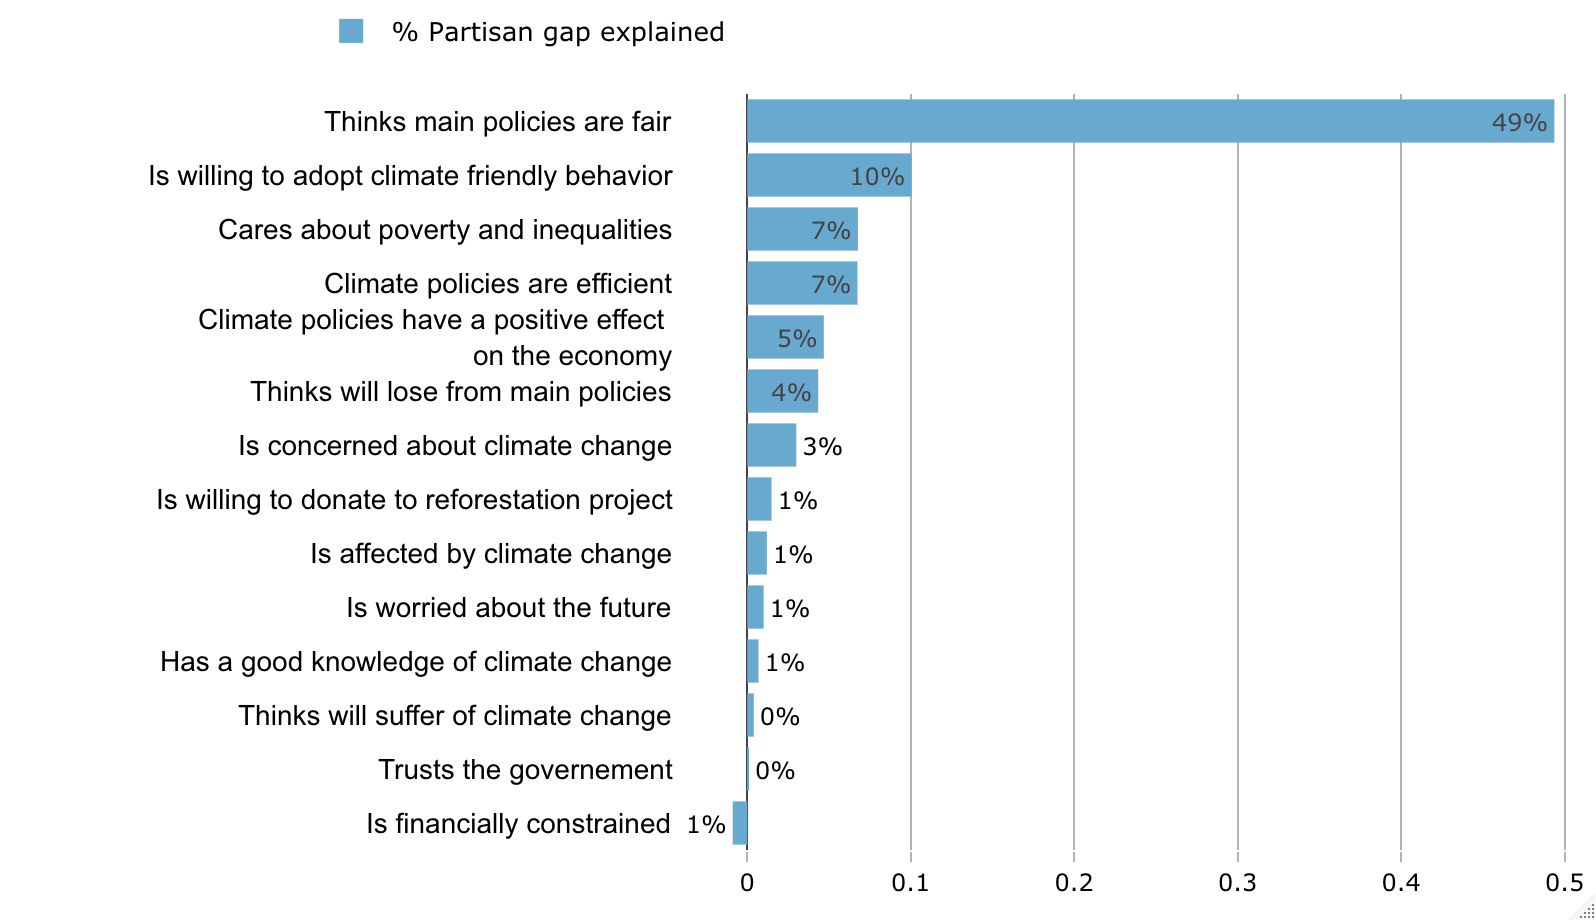
\includegraphics[width=\textwidth]{gelbach_right_standard_D2SD}
		\end{subfigure}&
		\begin{subfigure}{0.5\textwidth}
		\caption{Carbon tax with cash transfers}
			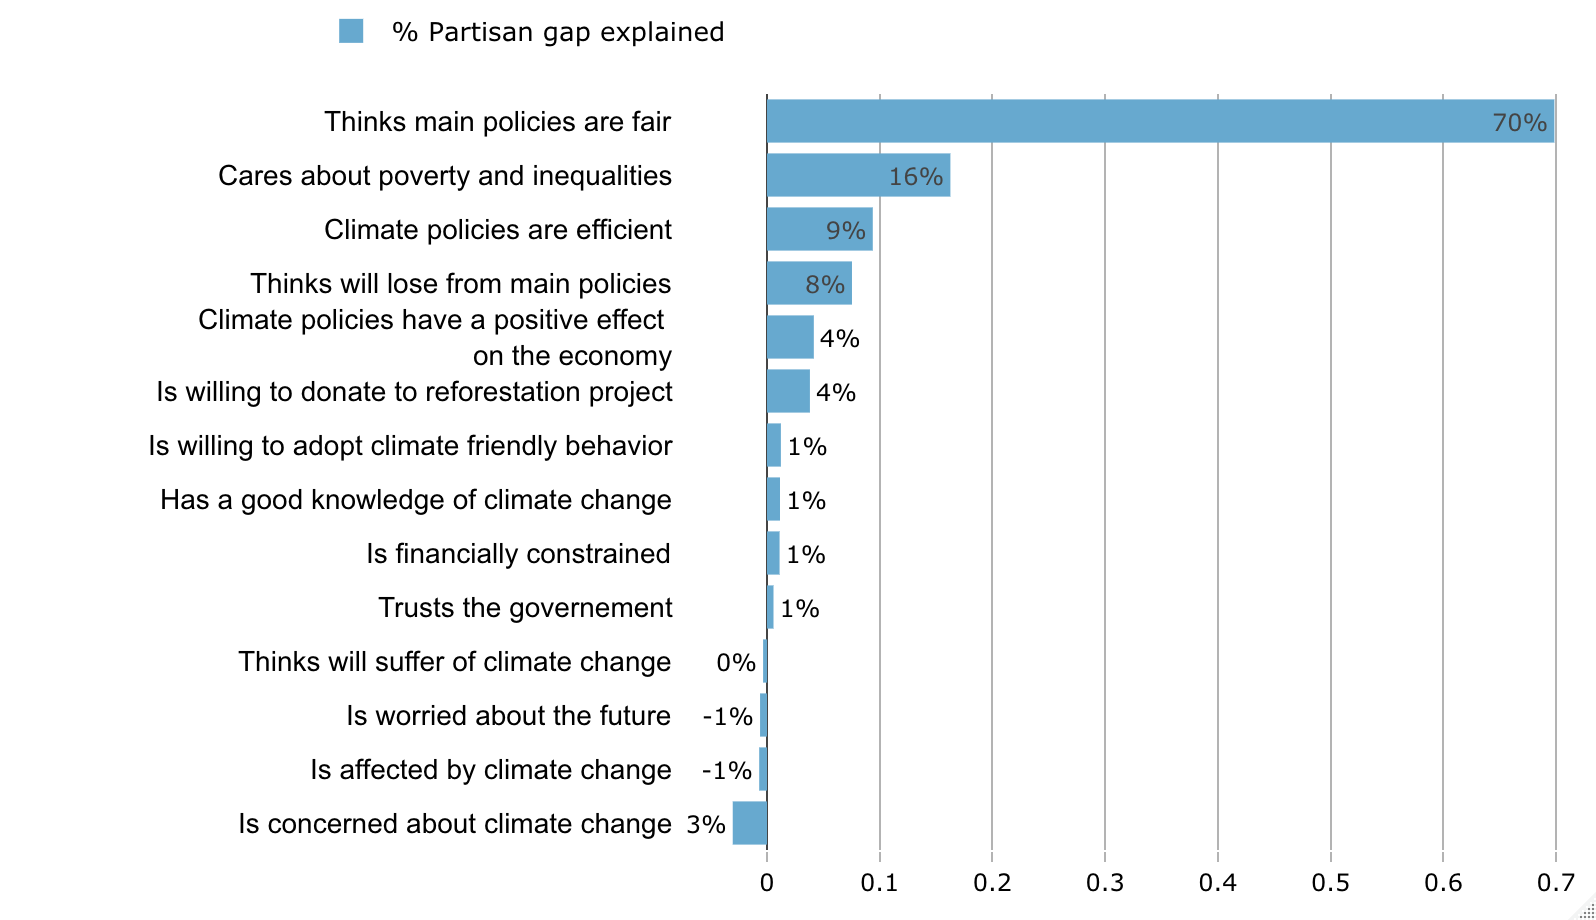
\includegraphics[width=\textwidth]{gelbach_right_tax_transfers_D2SD}
		\end{subfigure}\\
	\end{tabular}

	\begin{tabular}{cc}
		\begin{subfigure}{0.5\textwidth}
		\caption{Green investment program}
			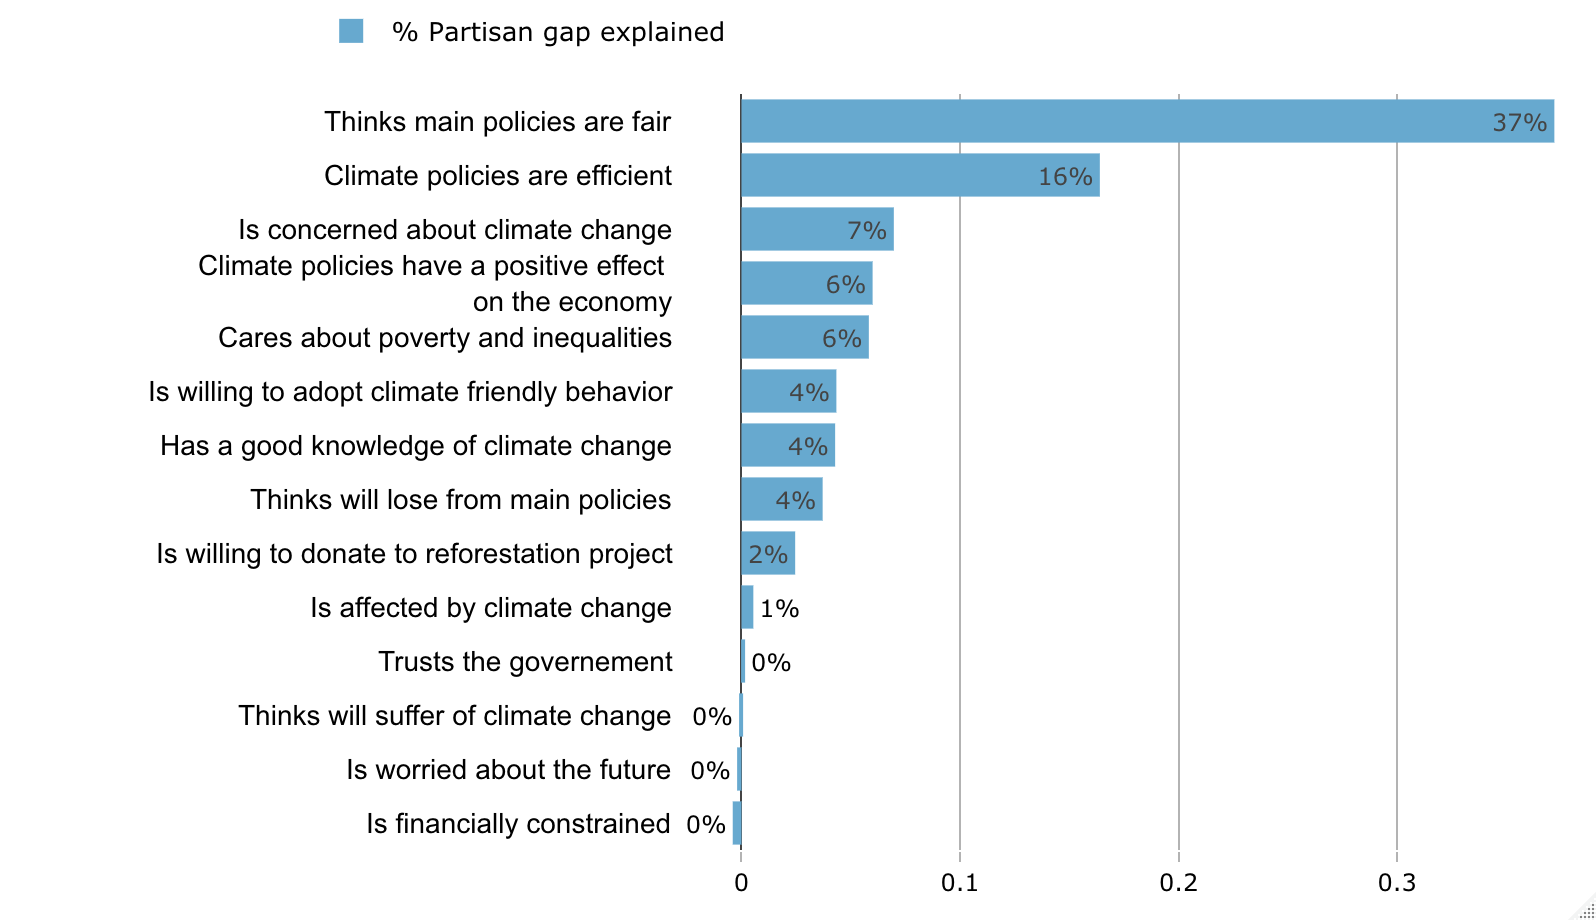
\includegraphics[width=\textwidth]{gelbach_right_investments_D2SD}
		\end{subfigure}&
		\begin{subfigure}{0.5\textwidth}
		\caption{All 3 policies}
			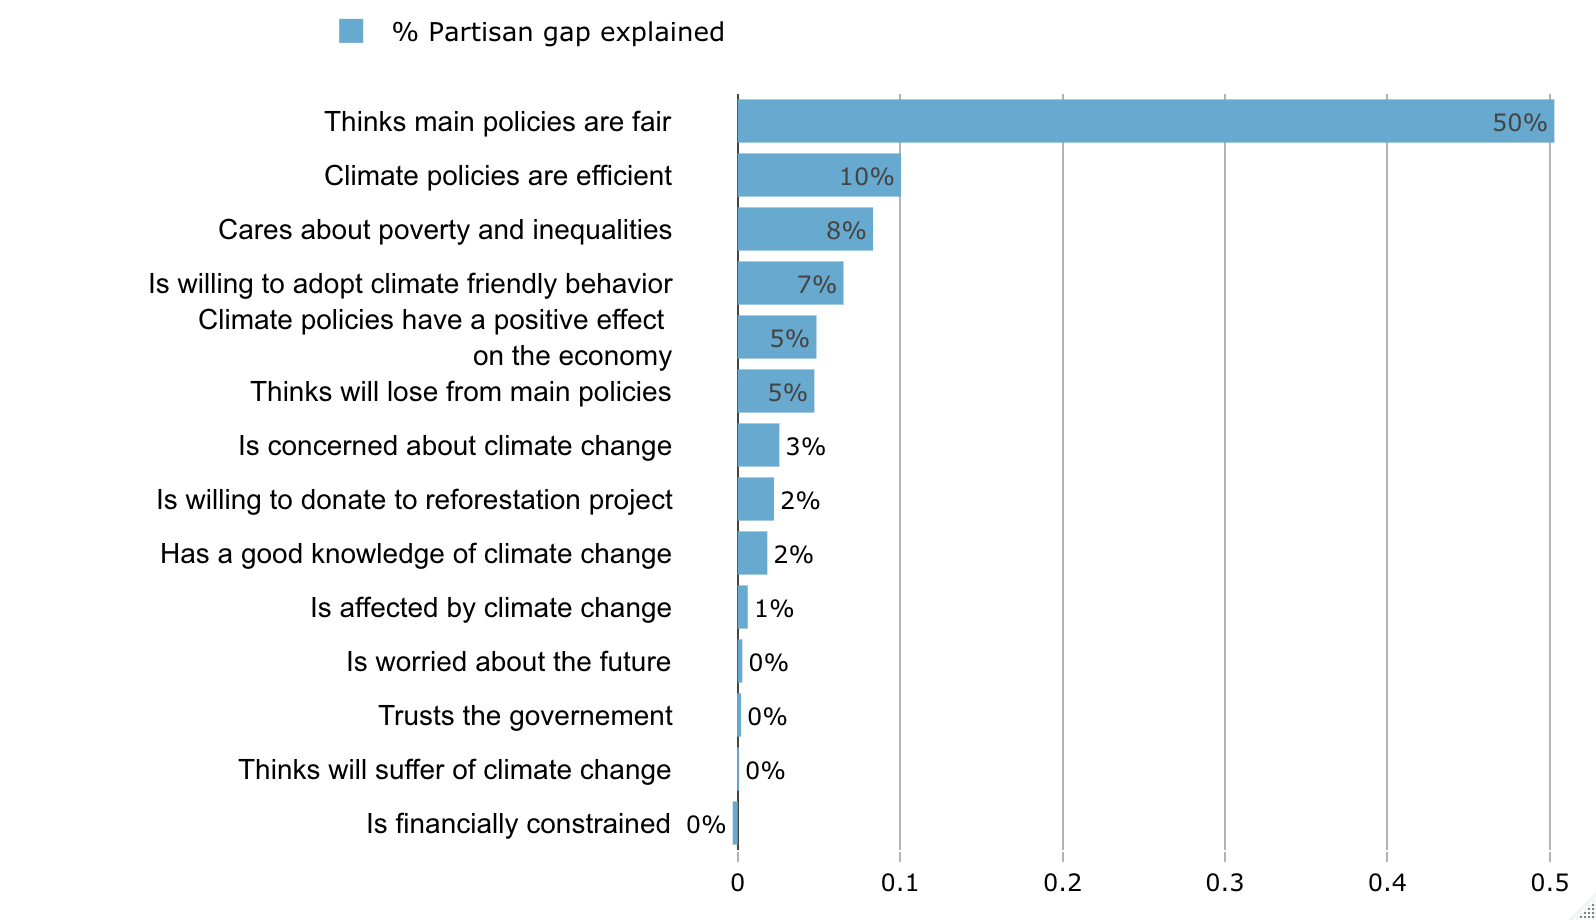
\includegraphics[width=\textwidth]{gelbach_right_main_policies_D2SD}
		\end{subfigure}\\
	\end{tabular}
		\end{center}

\end{figure}


\begin{figure}[h!]
	\caption{Gelbach decomposition of the partisan gap in support for all climate policies}	
		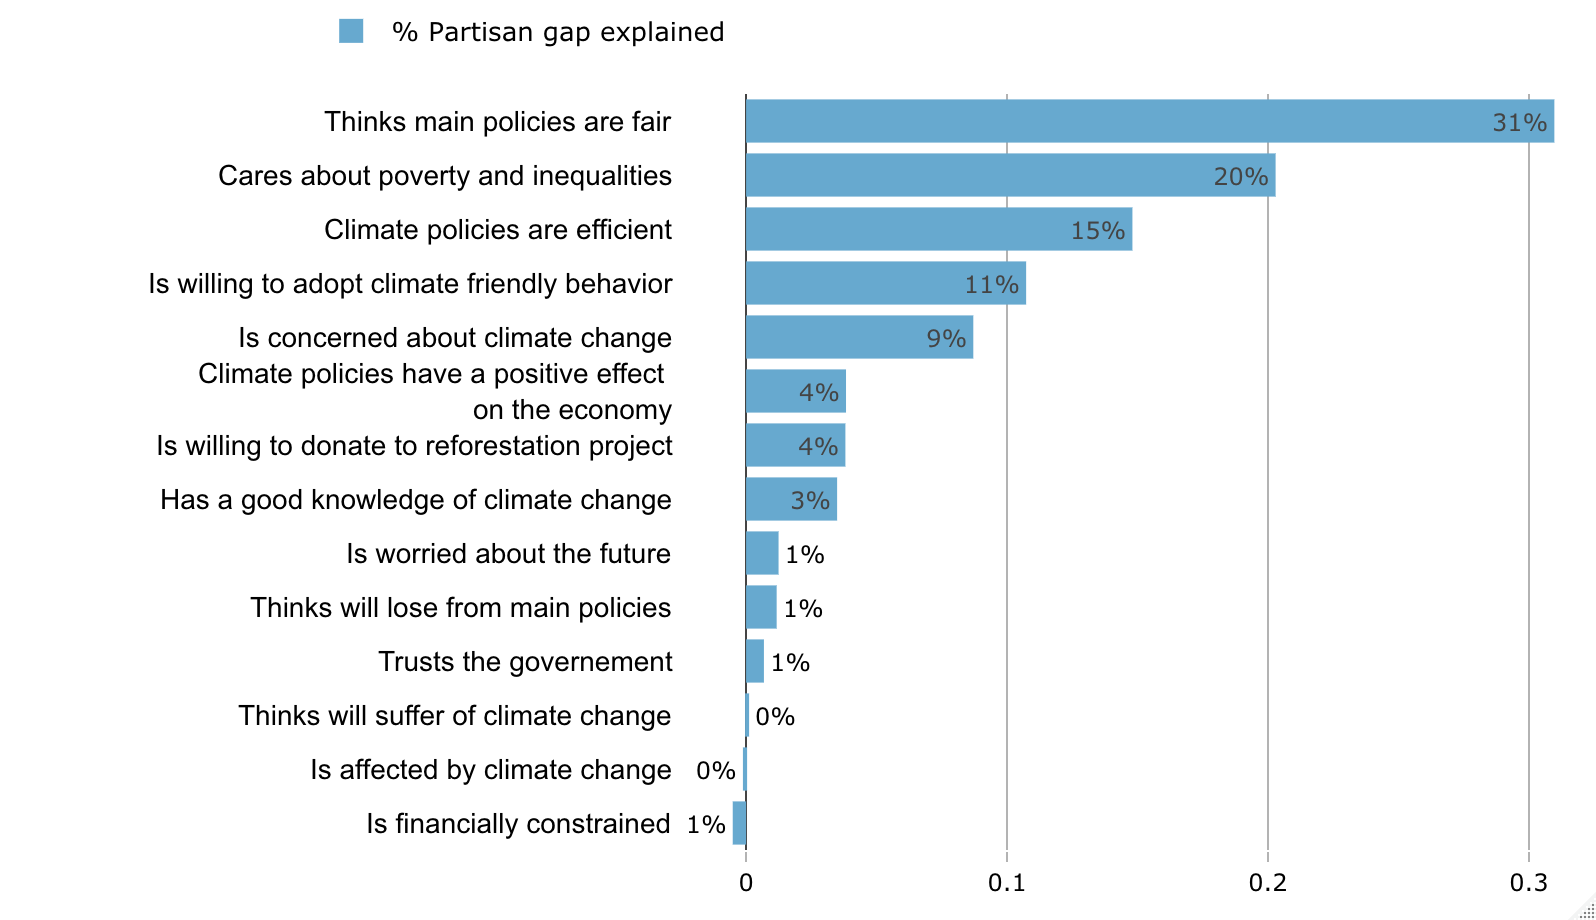
\includegraphics[width=\textwidth]{gelbach_right_all_policies_D2SD}
\end{figure}


\begin{figure}[h!]
\begin{center}
	\caption{Explaining the Geographical Gap}
	\caption*{Gelbach decomposition of the geographical gap (urban vs. rural) in support for:}
	\setlength\extrarowheight{-1pt}
	\begin{tabular}{cc}
		\begin{subfigure}{0.5\textwidth}
		\caption{Ban on combustion-engine cars}
			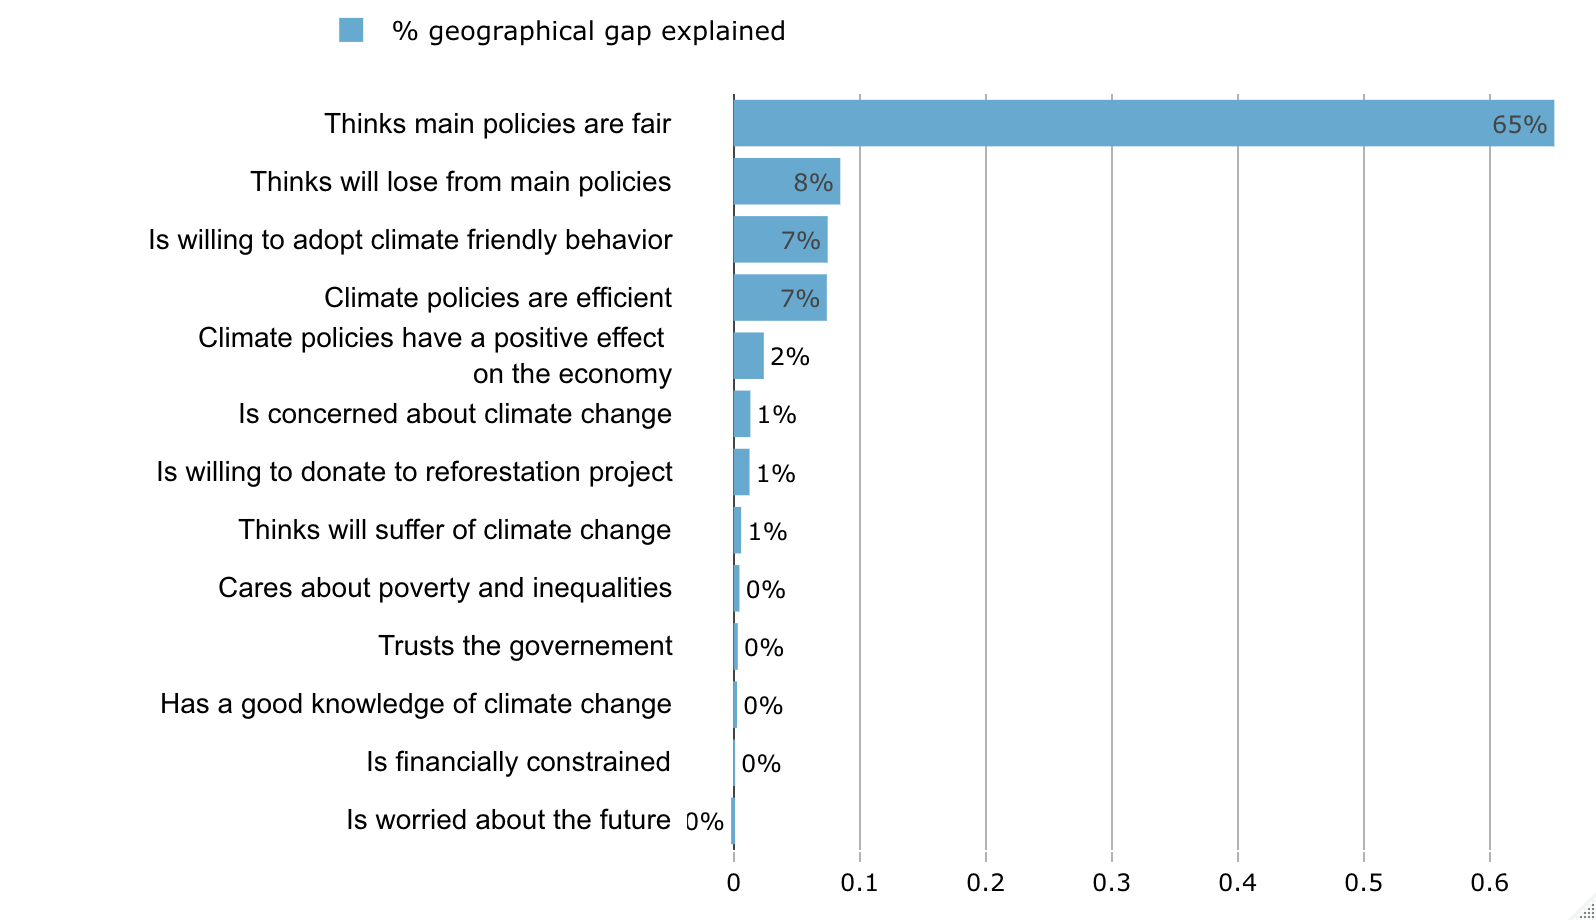
\includegraphics[width=\textwidth]{gelbach_urban_standard_D2SD}
		\end{subfigure}&
		\begin{subfigure}{0.5\textwidth}
		\caption{Carbon tax with cash transfers}
			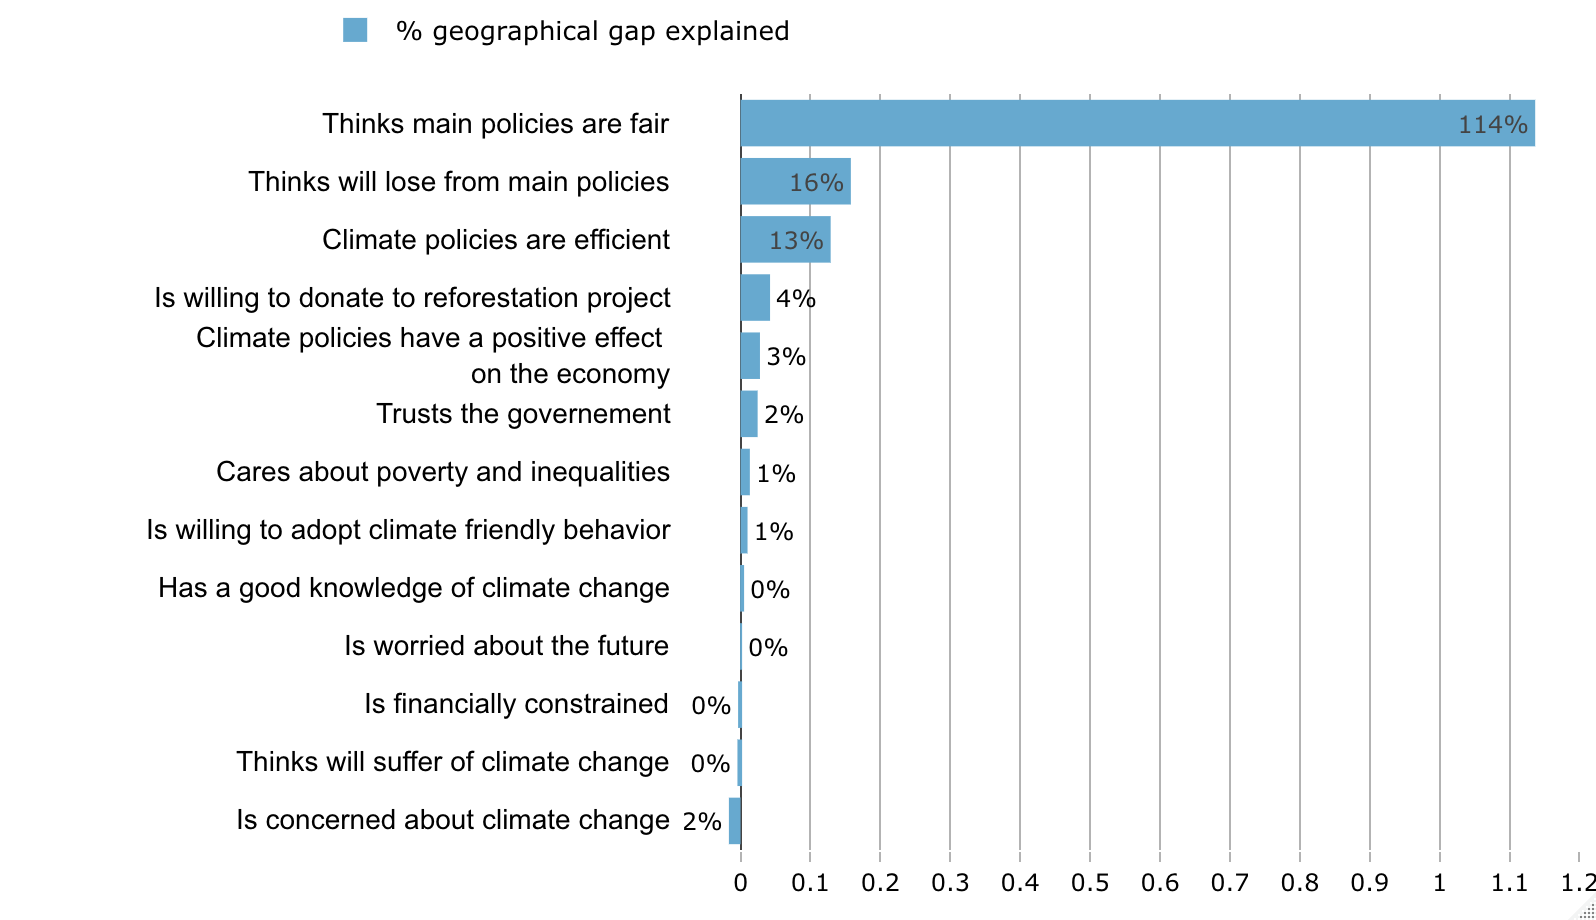
\includegraphics[width=\textwidth]{gelbach_urban_tax_transfers_D2SD}
		\end{subfigure}\\
	\end{tabular}

	\begin{tabular}{cc}
		\begin{subfigure}{0.5\textwidth}
		\caption{Green investment program}
			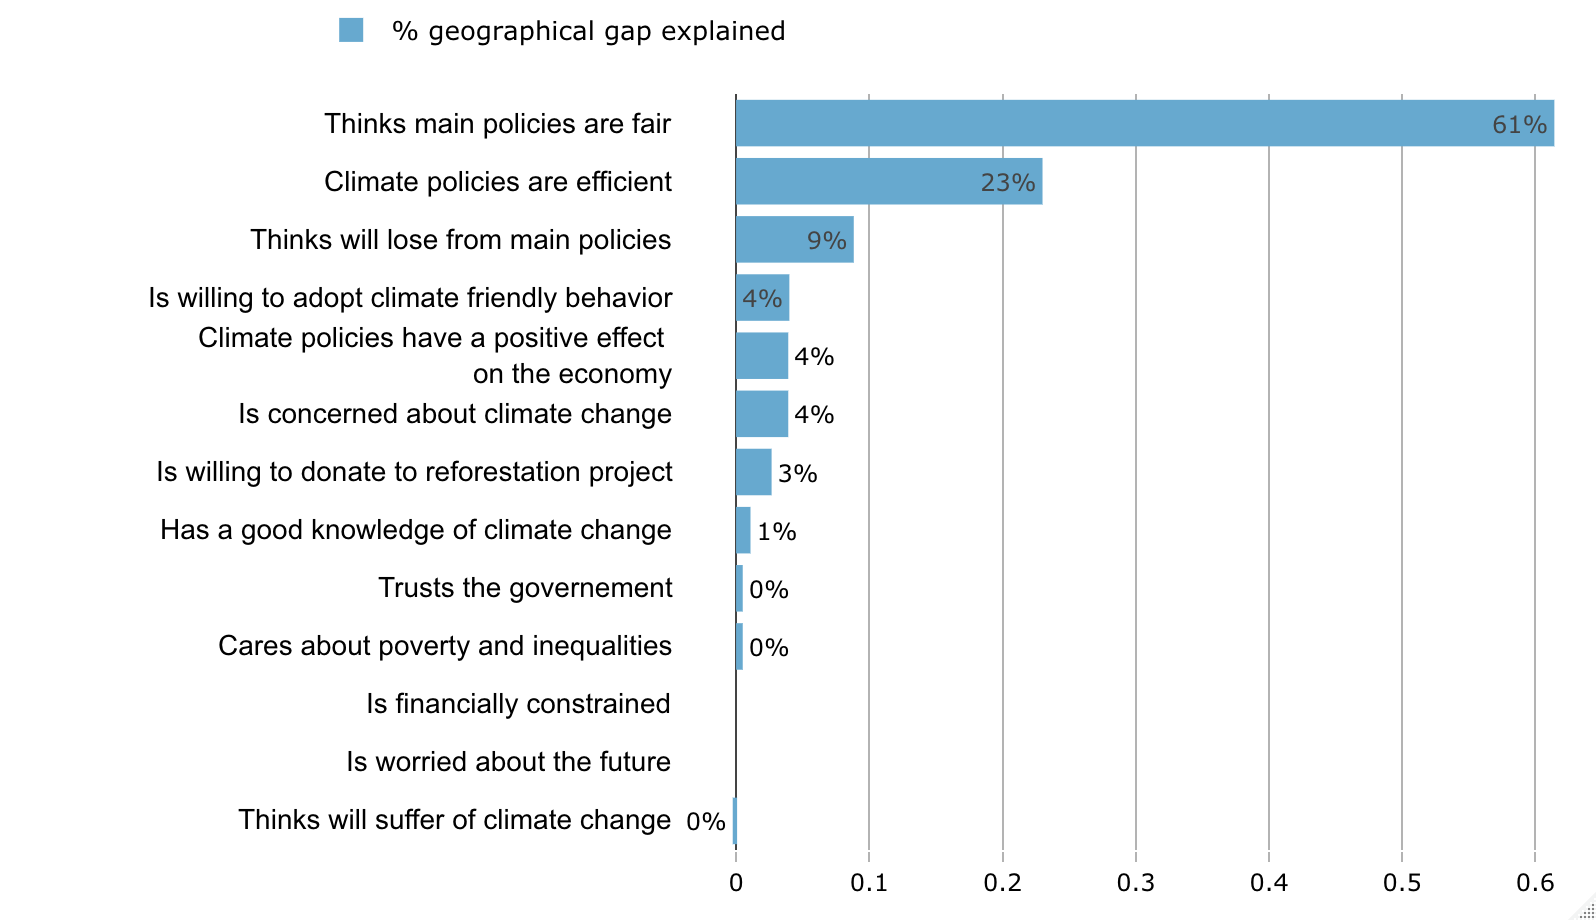
\includegraphics[width=\textwidth]{gelbach_urban_investments_D2SD}
		\end{subfigure}&
		\begin{subfigure}{0.5\textwidth}
		\caption{All 3 policies}
			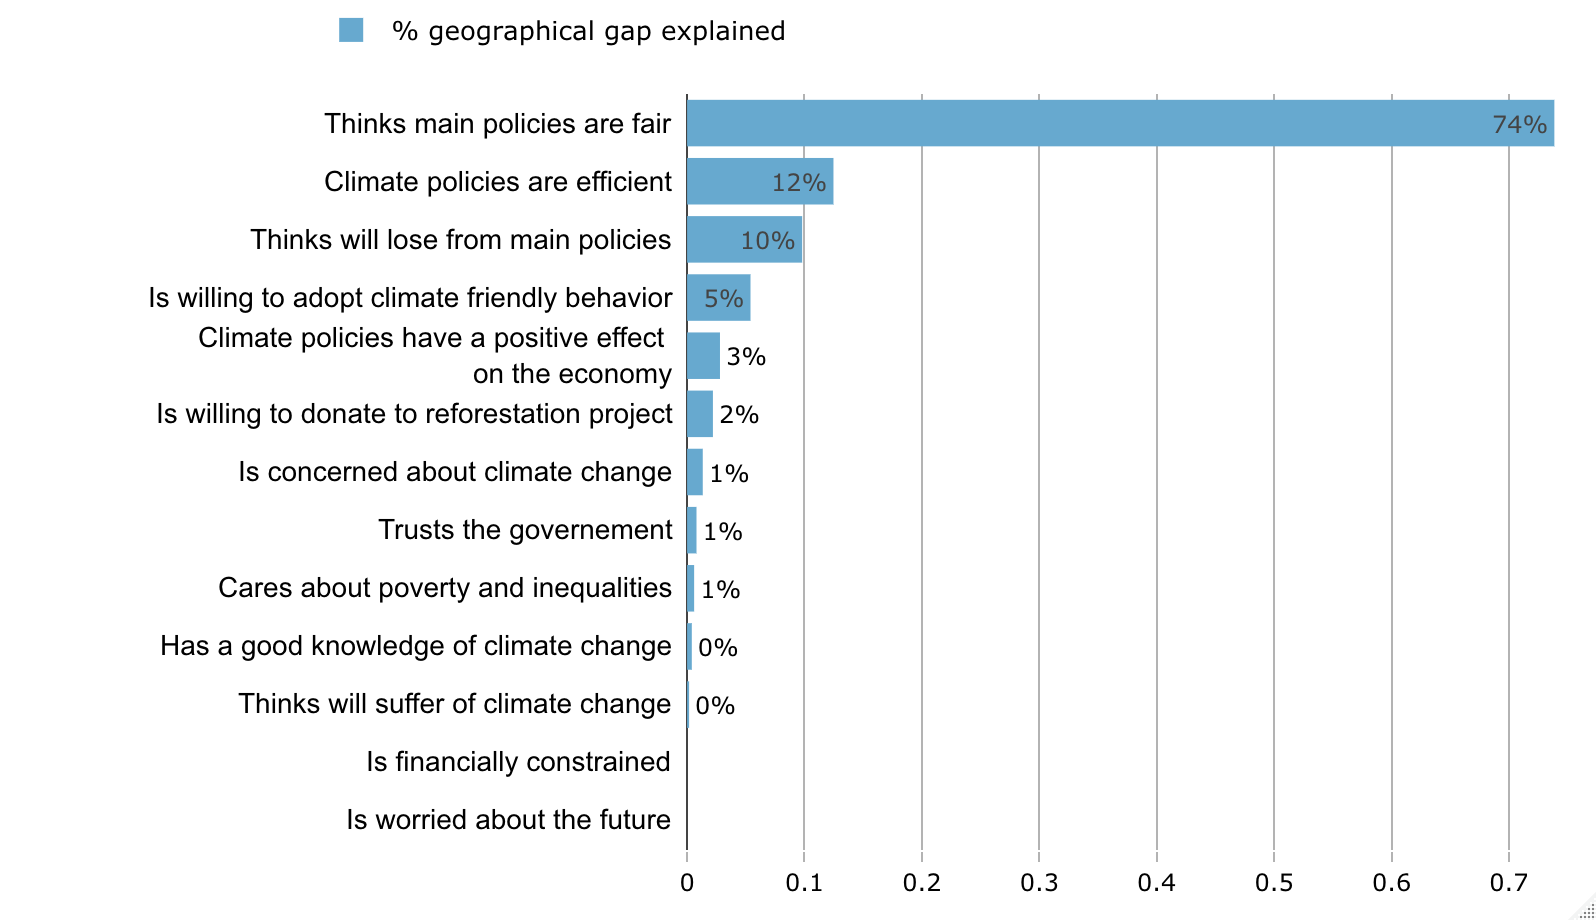
\includegraphics[width=\textwidth]{gelbach_urban_main_policies_D2SD}
		\end{subfigure}\\
	\end{tabular}
		\end{center}

\end{figure}


\begin{figure}[h!]
	\caption{Gelbach decomposition of the geographical gap (urban vs. rural) in support for all climate policies}	
		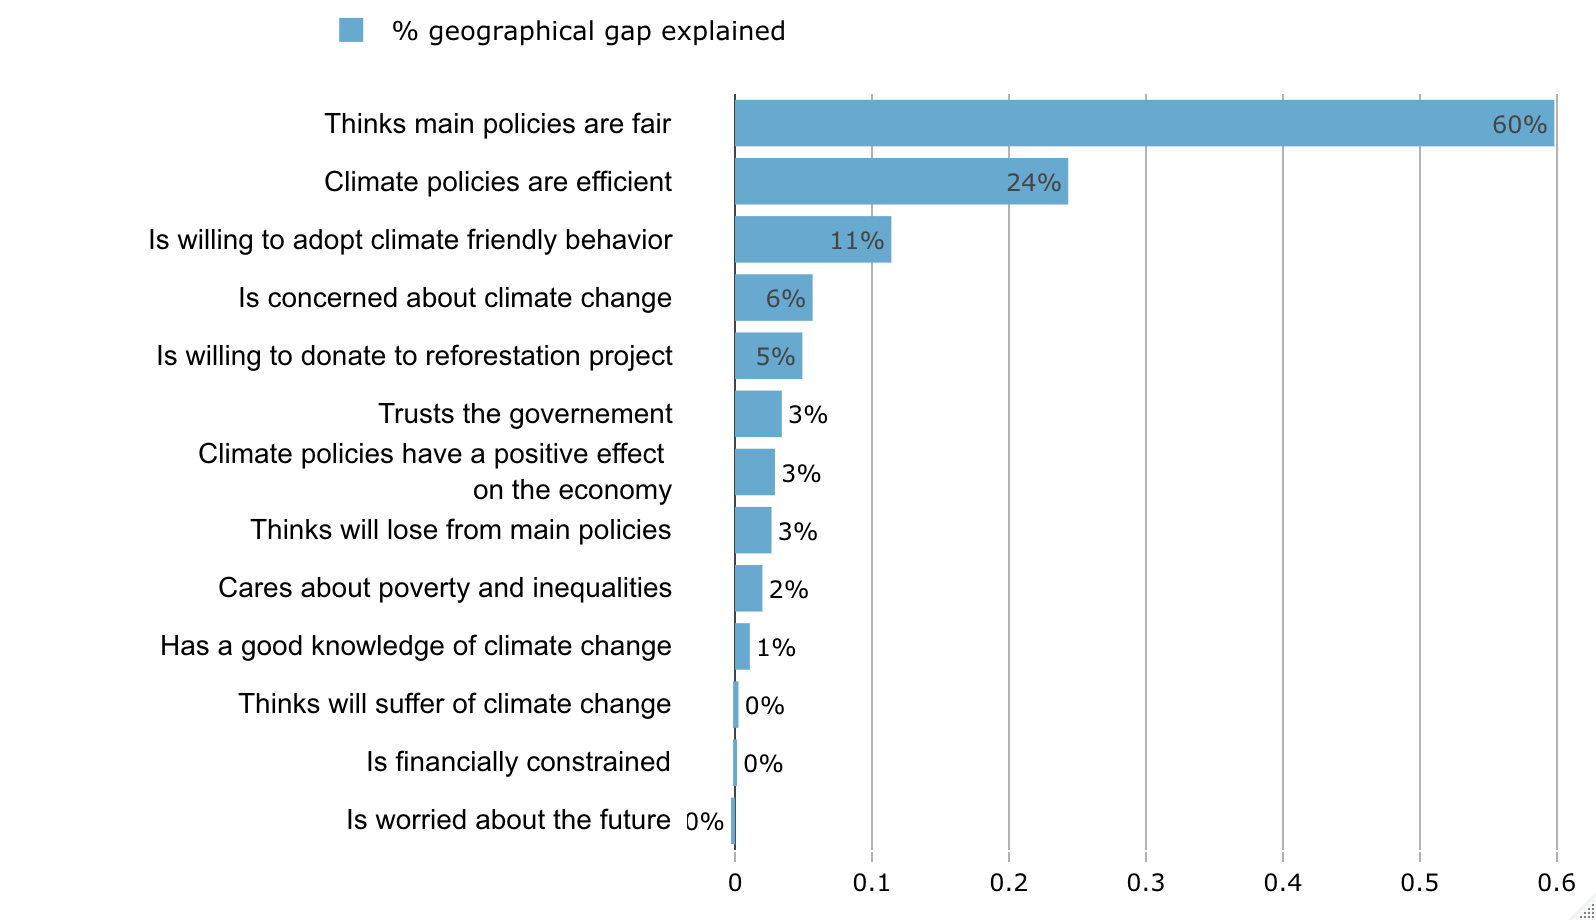
\includegraphics[width=\textwidth]{gelbach_urban_all_policies_D2SD}
\end{figure}

\end{document}